\chapter{Java Input and Output}
An early \nr{} design decision was to leave I/O operations out of the
language, and to depend on the JVM functionality for this. This
turned out to be a mixed blessing, as JVM I/O has been enhanced and
changed over the years; on the other hand, JVM I/O has changed (and
grown) a lot
over the years, and did become a complex component. Also, the various environments in which \nr{}
can be used as a programming language, are not limited to file I/O,
but have various implementations to interact with the outside world. A
\nr{} program that employs Web technology has different method calls
to make than a program that uses ISPF for user interaction.

% This does not preclude us to implement file I/O in a way that is
% reminiscent of Classic \Rexx{}, and in fact this has been done, and
% the future might see a compatible implementation in \nr{}.


\section{The File Class}
The Java \keyword{File} class represents a file\footnote{or rather a path}; various pieces of
information can be requested from a instance of this class, when it
points to a file on disk.

  \subsection{Example}
  \lstinputlisting[label=linecomment,caption=Buffered I?O]{../../../../examples/NrxRedBk/file/FileInfo.nrx}
% \section{Streams}
% \section{Line mode I/O}
% \subsection{Line mode I/O using BufferedReader and PrintWriter}
  \subsection{Line mode I/O using BufferedReader and FileOutputStream}
  While standard Java I/O does not perform particularly well in the
  unbuffered version, a \keyword{BufferedReader} can be wrapped around
  any \keyword{Reader} in order to maximize the amount of data that is
  read in one I/O operation.
  \subsubsection{Example}
\lstinputlisting[label=linecomment,caption=Buffered I?O]{../../../../examples/ibm-historic/linecomment.nrx}
% \section{Byte Oriented I/O}

% \section{Data Oriented I/O}
\section{Object Oriented I/O using Serialization}
The serialization methods of a Class can be used to write a class as
serialized binary data. Using the \keyword{writeObject()} method, an
object can be written to a file using one call. Note that the \Rexx{}
class is serializable for a long time already.
\subsection{Example}
\lstinputlisting[label=linecomment,caption=Buffered I?O]{../../../../examples/NrxRedBk/file/SeriaIO.nrx}
% \section{The NIO Approach}



\section{Using the SAY instruction to write lines to a file}
It used to be that a lot of programs started out with using
\keyword{say} statements to write to the console, and later, when
output became too voluminous, needed to be reworked to use output
statements. \keyword{Say} has been extended to write to any (and
multiple) outputstream(s).

The \keyword{setOutputStream()} Method takes an \emph{OutputStream} which
from that moment on is used for output. This can be
\keyword{System.out} (which is the default) but also
\keyword{System.err}, to direct error messages to. This outputstream
can also be directed to a file, using a \keyword{FileOutputStream}.

In addition to the \keyword{setOutputStream()} operation, which
replaces the previously set \emph{OutputStream}, there are
also \keyword{pushOutputStream()} and \keyword{popOutputStream()},
which add (push) and remove (pop) streams from a list. In this way, it
is possible to direct output to, e.g. an System.out and System.err
stream, and at the same time to a number of files.

These operations are not a good fit for multithreaded programs. For
use in the heavily multithreaded Pipelines environment, the method
\keyword{RexxIO.pipeSay} was designed, which is used in the Pipelines
source code, but can also be employed in your own multithreaded programs.
\subsubsection{Example}
\lstinputlisting{../../../../examples/new-3.07/pushpop.nrx}


\section{Using RexxIO.forEachLine }

A pattern in which there is an action for every line in a file, is now supported with the oneliner
file handler, RexxIO.forEachLine. A Class that implements the
interface \keyword{LineHandler} can read lines from a file using the \\
\keyword{RexxIO().File('filename').forEachLine(x)} idiom, which is
very compact. The \keyword{LineHandler} interface needs to implement
the \keyword{handle()} method, which is fed the line that has been read.

\subsubsection{Example}

\lstinputlisting[label=linecomment,caption=Buffered I?O]{../../../../examples/new-3.07/testLine.nrx}
% This is shown in the figures \ref{fig:3.07.1}, \ref{fig:3.07.2} and \ref{fig:3.07.3}.

% \begin{figure*}[h]
%     \begin{center}
%       \scalebox{0.2}{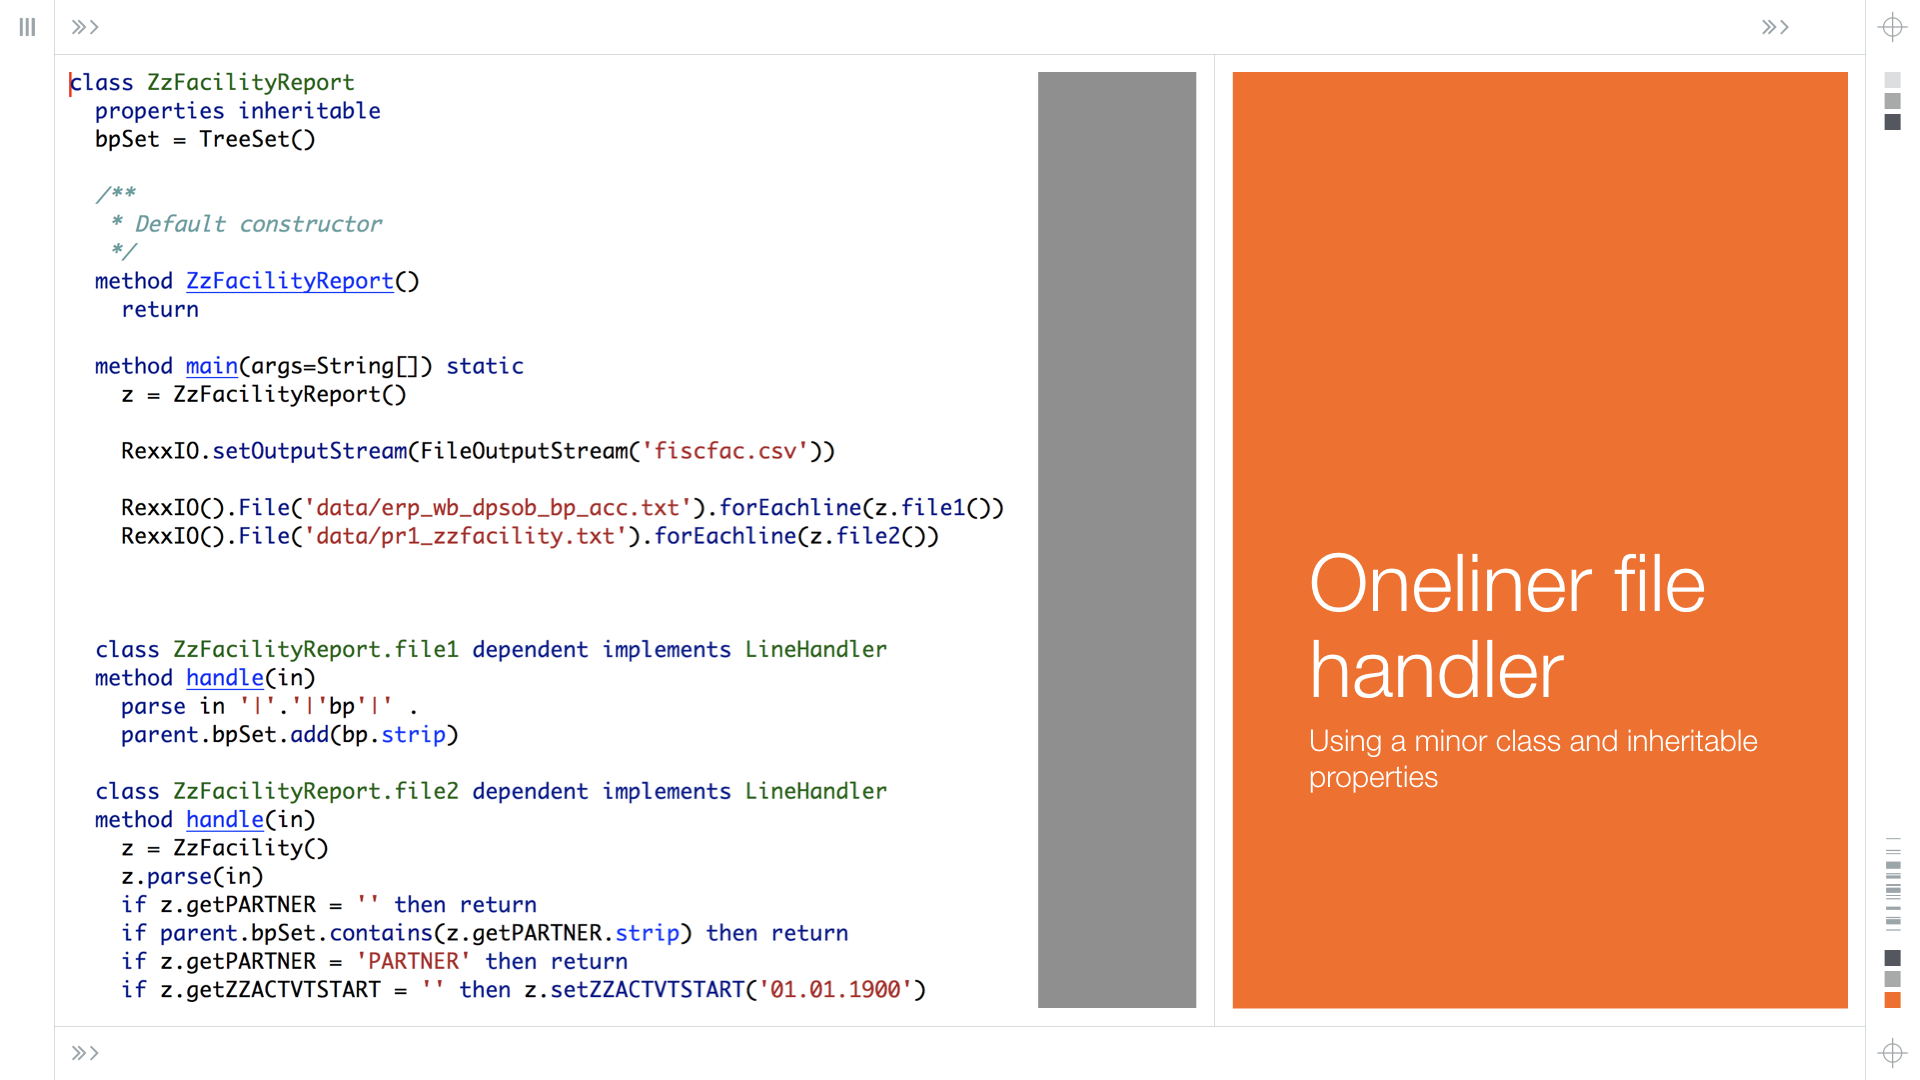
\includegraphics{NetRexx3.07.008.png}}
%     \end{center}
%     \caption{Oneliner file handler} \label{fig:3.07.1}
%   \end{figure*}

% \begin{figure*}[h]
%     \begin{center}
%       \scalebox{0.2}{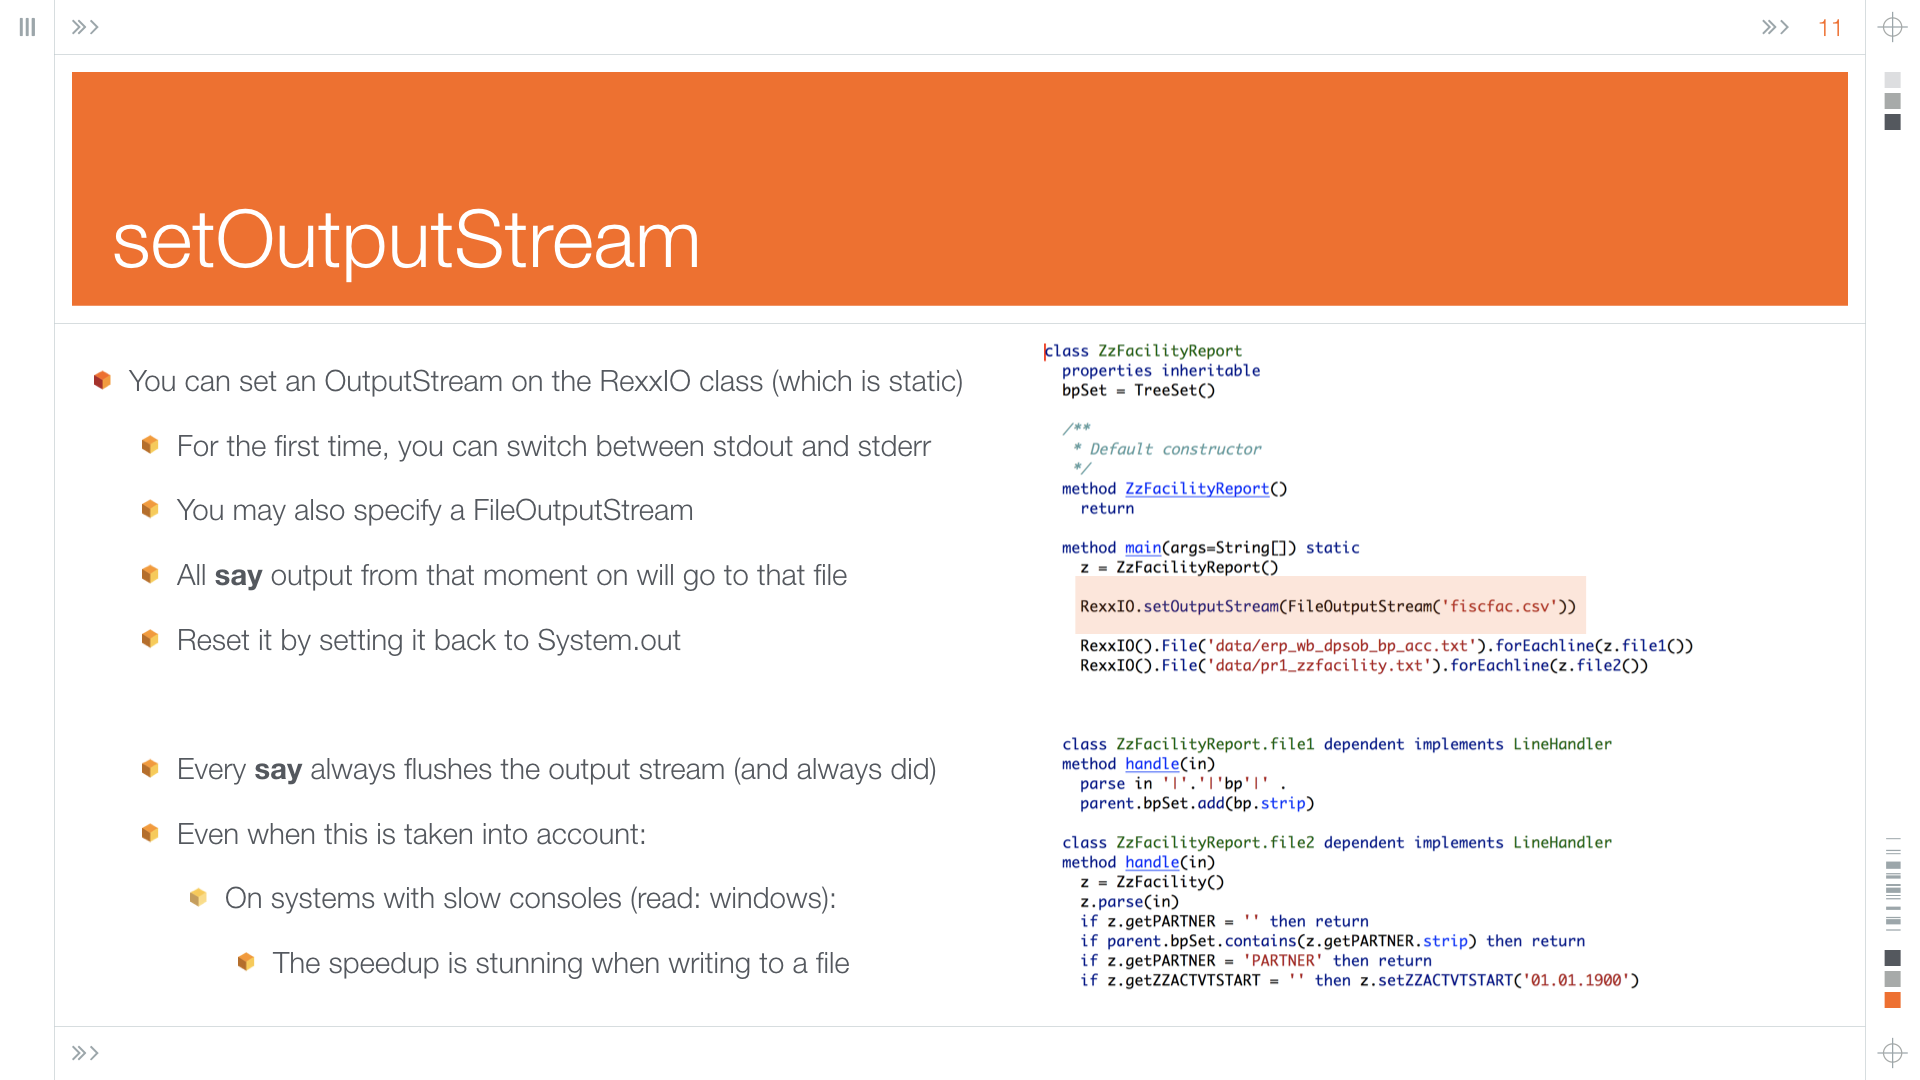
\includegraphics{NetRexx3.07.011.png}}
%     \end{center}
%     \caption{Set the output stream for Say} \label{fig:3.07.2}
%   \end{figure*}

% \begin{figure*}[h]
%     \begin{center}
%       \scalebox{0.2}{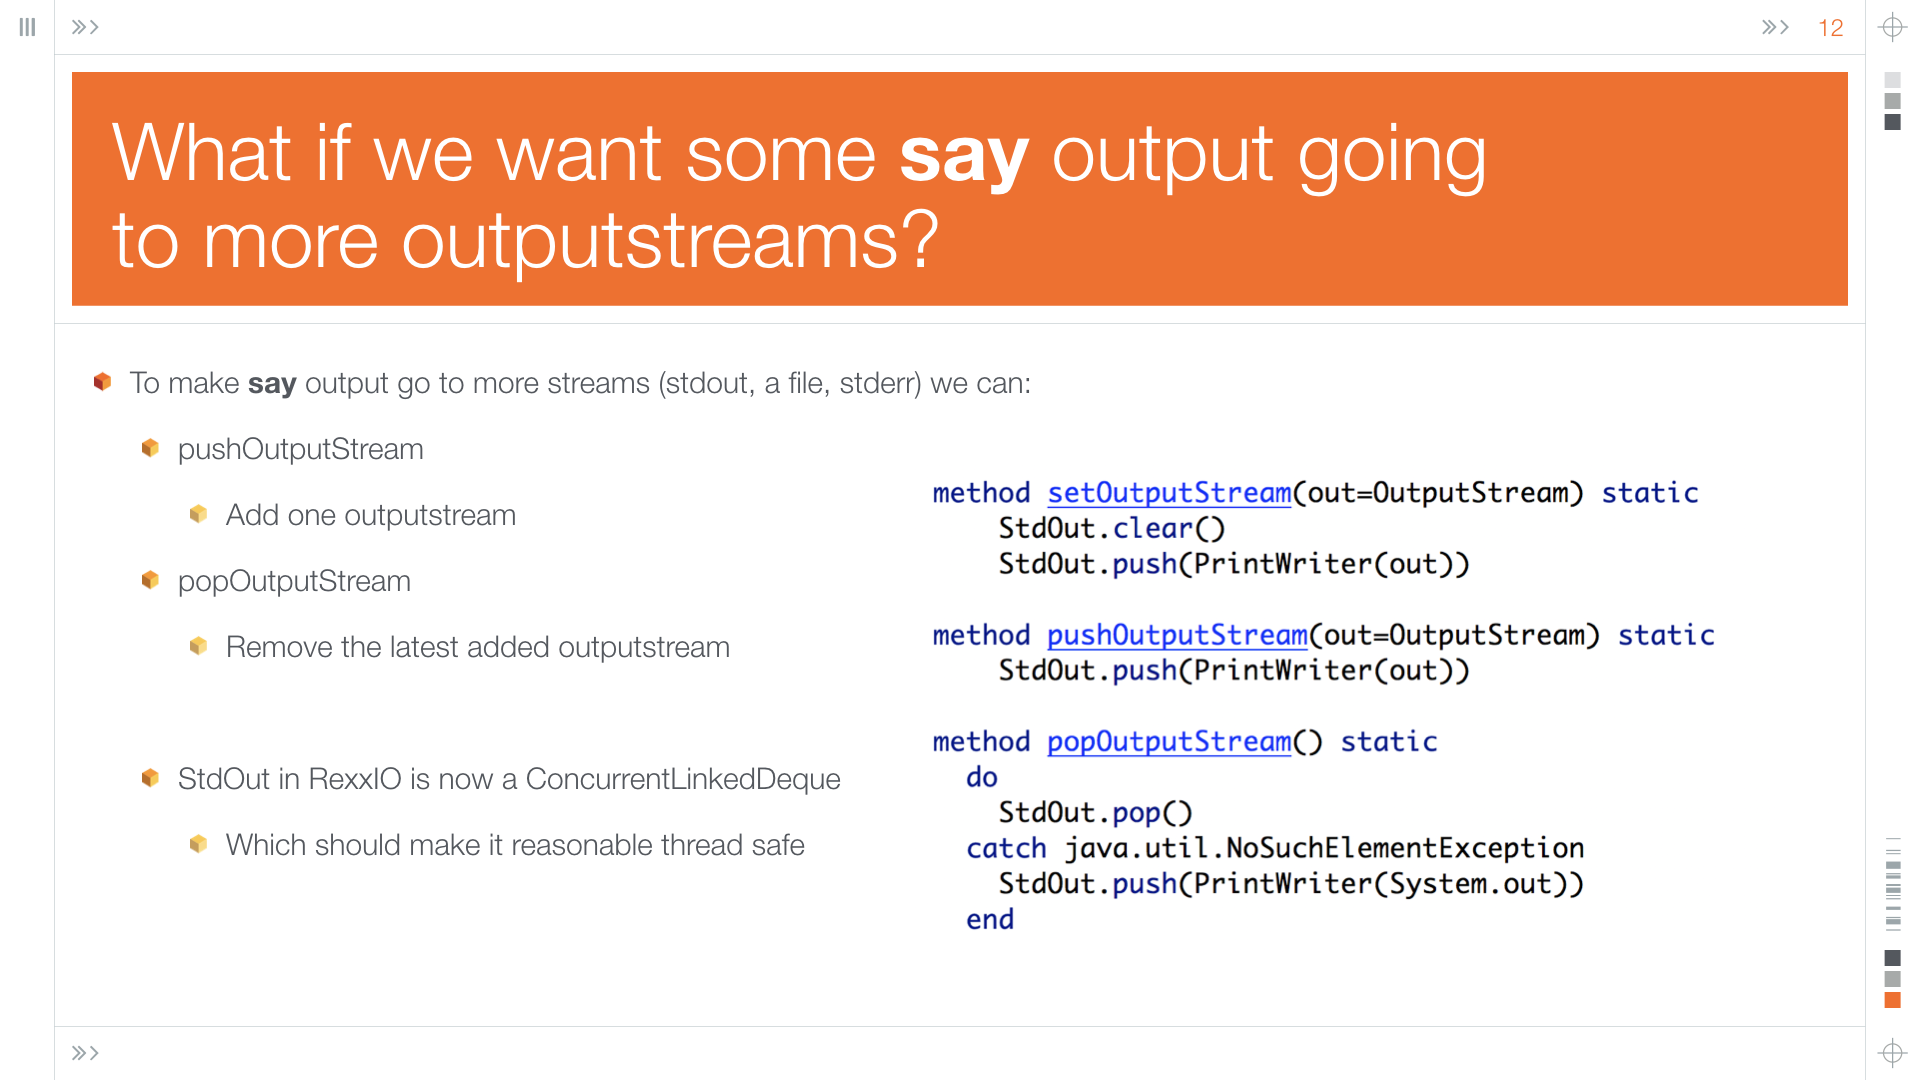
\includegraphics{NetRexx3.07.012.png}}
%     \end{center}
%     \caption{Using more outputstreams} \label{fig:3.07.3}
%   \end{figure*}

